% answers.tex —— 2004 年·春季北京卷·文科 · 参考答案与详细解析片段
% 由 tools/generate_projects.py 依来源总账自 2004/2004_数学真题_春季北京文_试题.md + 2004/2004_数学真题_春季北京文_解析正文.md + 2004/2004_数学真题_春季北京文_答案要点.md 生成，勿手改（改源 MD 后重跑）


\begin{gktip}
以下解析是主会话的独立推导，不是来源印载解析。已有一名复核者仅据固定 PDF 独立解答 Q1–Q20；其 Q16 最终数值与中间推导矛盾，主会话复算确认本稿结论 $\sqrt3/2$ 正确。计算过程依据当前题面转录；固定 PDF 仅绑定为本库内部 canonical 输入，题面文字逐页独立复核已完成，Q20源文疑脱仍未核定；来源出版信息及官方身份仍未认证。
\end{gktip}

\begin{answer}
\gksolhead{1}{}

\textbf{题目}：

在函数 $y=\sin 2x$、$y=\sin x$、$y=\cos x$、$y=\tan\dfrac{x}{2}$ 中，最小正周期为 $\pi$ 的函数是\mbox{（　　）}。

（A）$y=\sin 2x$　　（B）$y=\sin x$　　（C）$y=\cos x$　　（D）$y=\tan\dfrac{x}{2}$

\Needspace{4\baselineskip}
\textbf{解析}

正弦、余弦函数 $\sin 2x$ 的最小正周期为 $\pi$；$\sin x$、$\cos x$ 的周期为 $2\pi$，$\tan(x/2)$ 的周期为 $2\pi$。故选 A。

\gkanswer{答案：A。}

\end{answer}
\begin{answer}
\gksolhead{2}{}

\textbf{题目}：

当 $m<1$ 时，复数 $z=2+(m-1)i$ 在复平面上对应的点位于\mbox{（　　）}。

（A）第一象限　　（B）第二象限　　（C）第三象限　　（D）第四象限

\Needspace{4\baselineskip}
\textbf{解析}

复数对应点为 $(2,m-1)$。实部 $2>0$，且 $m<1$ 使虚部 $m-1<0$，所以点在第四象限，选 D。

\gkanswer{答案：D。}

\end{answer}
\begin{answer}
\gksolhead{3}{}

\textbf{题目}：

双曲线 $\dfrac{x^2}{4}-\dfrac{y^2}{9}=1$ 的渐近线方程是\mbox{（　　）}。

（A）$y=\pm\dfrac{3}{2}x$　　（B）$y=\pm\dfrac{2}{3}x$　　（C）$y=\pm\dfrac{9}{4}x$　　（D）$y=\pm\dfrac{4}{9}x$

\Needspace{4\baselineskip}
\textbf{解析}

双曲线 $\dfrac{x^2}{4}-\dfrac{y^2}{9}=1$ 的半实轴长 $a=2$、半虚轴长 $b=3$，渐近线为 $y=\pm\dfrac ba x=\pm\dfrac32x$，选 A。

\gkanswer{答案：A。}

\end{answer}
\begin{answer}
\gksolhead{4}{}

\textbf{题目}：

一个圆锥的侧面积是其底面积的 $2$ 倍，则该圆锥的母线与底面所成的角为\mbox{（　　）}。

（A）$30^\circ$　　（B）$45^\circ$　　（C）$60^\circ$　　（D）$75^\circ$

\Needspace{4\baselineskip}
\textbf{解析}

设圆锥底面半径为 $r$、母线长为 $l$。侧面积为 $\pi rl$，底面积为 $\pi r^2$，条件给出 $l=2r$。若母线与底面夹角为 $\varphi$，母线在底面上的投影长为 $r$，因此 $\cos\varphi=r/l=1/2$，得 $\varphi=60^\circ$，选 C。

\gkanswer{答案：C，即 $60^\circ$。}

\end{answer}
\begin{answer}
\gksolhead{5}{}

\textbf{题目}：

已知 $\sin(\theta+\pi)<0$，$\cos(\theta-\pi)>0$，则下列不等关系中必定成立的是\mbox{（　　）}。

（A）$\sin\theta<0$，$\cos\theta>0$　　（B）$\sin\theta>0$，$\cos\theta<0$

（C）$\sin\theta>0$，$\cos\theta>0$　　（D）$\sin\theta<0$，$\cos\theta<0$

\Needspace{4\baselineskip}
\textbf{解析}

由 $\sin(\theta+\pi)=-\sin\theta<0$ 得 $\sin\theta>0$；由 $\cos(\theta-\pi)=-\cos\theta>0$ 得 $\cos\theta<0$。对应选项 B。

\gkanswer{答案：B。}

\end{answer}
\begin{answer}
\gksolhead{6}{}

\textbf{题目}：

在抛物线 $y^2=2px$ 上，横坐标为 $4$ 的点到焦点的距离为 $5$，则 $p$ 的值为\mbox{（　　）}。

（A）$\dfrac12$　　（B）$1$　　（C）$2$　　（D）$4$

\Needspace{4\baselineskip}
\textbf{解析}

抛物线 $y^2=2px$ 的焦点为 $(p/2,0)$。抛物线上横坐标为 $4$ 的点到焦点的距离等于其到准线 $x=-p/2$ 的距离，即 $4+p/2$。于是 $4+p/2=5$，解得 $p=2$，选 C。

\gkanswer{答案：C，即 $p=2$。}

\end{answer}
\begin{answer}
\gksolhead{7}{}

\textbf{题目}：

已知 $a,b,c,d$ 均为实数，有下列命题：

① 若 $ab>0$，$bc-ad>0$，则 $\dfrac{c}{a}-\dfrac{d}{b}>0$；

② 若 $ab>0$，$\dfrac{c}{a}-\dfrac{d}{b}>0$，则 $bc-ad>0$；

③ 若 $bc-ad>0$，$\dfrac{c}{a}-\dfrac{d}{b}>0$，则 $ab>0$。

其中正确命题的个数是\mbox{（　　）}。

（A）$0$　　（B）$1$　　（C）$2$　　（D）$3$

\Needspace{4\baselineskip}
\textbf{解析}

\Needspace{5\baselineskip}
因题中分式有定义，$a,b\ne0$，并且
\nopagebreak[4]
\[
\frac ca-\frac db=\frac{bc-ad}{ab}.
\]
①在 $ab>0$、$bc-ad>0$ 时商为正，成立；②在 $ab>0$ 且商为正时，分子 $bc-ad>0$，成立；③已知分子为正且商为正，分母 $ab$ 必为正，成立。三个命题均正确，选 D。

\gkanswer{答案：D，三个命题都正确。}

\end{answer}
\begin{answer}
\gksolhead{8}{}

\textbf{题目}：

两个完全相同的长方体的长、宽、高分别为 $5\,\text{cm}$、$4\,\text{cm}$、$3\,\text{cm}$，把它们重叠在一起组成一个新长方体，在这些新长方体中，最长的对角线的长度是\mbox{（　　）}。

（A）$\sqrt{77}\,\text{cm}$　　（B）$7\sqrt2\,\text{cm}$　　（C）$5\sqrt5\,\text{cm}$　　（D）$10\sqrt2\,\text{cm}$

\Needspace{4\baselineskip}
\textbf{解析}

两长方体面贴合组成长方体时，可沿长、宽或高方向叠放，三种尺寸分别为 $(10,4,3)$、$(5,8,3)$、$(5,4,6)$。对应体对角线长为 $\sqrt{125}=5\sqrt5$、$\sqrt{98}=7\sqrt2$、$\sqrt{77}$。其中 $125$ 最大，故最长对角线是 $5\sqrt5\,\text{cm}$，选 C。

\gkanswer{答案：C，即 $5\sqrt5\,\text{cm}$。}

\end{answer}
\begin{answer}
\gksolhead{9}{}

\textbf{题目}：

在 $100$ 件产品中有 $6$ 件次品，现从中任取 $3$ 件产品，至少有 $1$ 件次品的不同取法的种数是\mbox{（　　）}。

（A）$\binom61\binom{94}2$　　（B）$\binom61\binom{99}2$　　（C）$A_{100}^3-A_{94}^3$　　（D）$\binom{100}3-\binom{94}3$

\Needspace{4\baselineskip}
\textbf{解析}

从 $100$ 件中取 $3$ 件的总数为 $\binom{100}{3}$；全部取自 $94$ 件正品的取法为 $\binom{94}{3}$。两者相减即至少含一件次品的取法数，选 D。

\gkanswer{答案：D，即 $\binom{100}{3}-\binom{94}{3}$。}

\end{answer}
\begin{answer}
\gksolhead{10}{}

\textbf{题目}：

期中考试以后，班长算出了全班 $40$ 个人数学成绩的平均分为 $M$。如果把 $M$ 当成一个同学的分数，与原来的 $40$ 个分数一起，算出这 $41$ 个分数的平均值为 $N$，那么 $M:N$ 为\mbox{（　　）}。

（A）$\dfrac{40}{41}$　　（B）$1$　　（C）$\dfrac{41}{40}$　　（D）$2$

\Needspace{4\baselineskip}
\textbf{解析}

原 $40$ 个分数之和为 $40M$。加入一个分数 $M$ 后，总和为 $41M$，平均值 $N=41M/41=M$，所以在题目所写比值有定义时，$M:N=1:1$，选 B。若 $M=0$，则仍有 $M=N$，但数值比 $0:0$ 无定义；这里按题目比值有定义的语境作答，不把 $M\ne0$ 补入原题。

\gkanswer{答案：B，即 $M:N=1:1$。}

\end{answer}
\begin{answer}
\gksolhead{11}{}

\textbf{题目}：

直线 $x-\sqrt3y+a=0$（$a$ 为常实数）的倾斜角的大小是 $\underline{\qquad}$。

\Needspace{4\baselineskip}
\textbf{解析}

直线写成 $y=\dfrac1{\sqrt3}x+\dfrac a{\sqrt3}$，斜率为 $1/\sqrt3$。倾斜角 $\alpha\in[0,\pi)$ 满足 $\tan\alpha=1/\sqrt3$，故 $\alpha=30^\circ$。

\gkanswer{答案：$30^\circ$。}

\end{answer}
\begin{answer}
\gksolhead{12}{}

\textbf{题目}：

$\dfrac{\sin(\alpha+30^\circ)-\sin(\alpha-30^\circ)}{\cos\alpha}$ 的值为 $\underline{\qquad}$。

\Needspace{4\baselineskip}
\textbf{解析}

\Needspace{5\baselineskip}
用差化积公式，
\nopagebreak[4]
\[
\sin(\alpha+30^\circ)-\sin(\alpha-30^\circ)
=2\cos\alpha\sin30^\circ=\cos\alpha.
\]
在原式有定义的条件 $\cos\alpha\ne0$ 下，所求值为 $1$。

\gkanswer{答案：$1$}

\end{answer}
\begin{answer}
\gksolhead{13}{}

\textbf{题目}：

若 $f^{-1}(x)$ 为函数 $f(x)=\lg(x-1)$ 的反函数，则 $f^{-1}(x)$ 的值域是 $\underline{\qquad}$。

\Needspace{4\baselineskip}
\textbf{解析}

由 $y=\lg(x-1)$ 得反函数 $f^{-1}(x)=10^x+1$，其值域为 $(1,+\infty)$。

\gkanswer{答案：$(1,+\infty)$。}

\end{answer}
\begin{answer}
\gksolhead{14}{}

\textbf{题目}：

若直线 $mx+ny-3=0$ 与圆 $x^2+y^2=3$ 没有公共点，则 $m,n$ 满足的关系式为 $\underline{\qquad}$；以 $(m,n)$ 为点 $P$ 的坐标，过点 $P$ 的一条直线与椭圆 $\dfrac{x^2}{7}+\dfrac{y^2}{3}=1$ 的公共点有 $\underline{\qquad}$ 个。

\Needspace{4\baselineskip}
\textbf{解析}

\Needspace{5\baselineskip}
原题称 $mx+ny-3=0$ 为直线，因此 $m^2+n^2>0$。圆心到直线的距离为
\nopagebreak[4]
\[
\frac3{\sqrt{m^2+n^2}}.
\]
没有公共点意味着距离严格大于圆半径 $\sqrt3$，因此 $m^2+n^2<3$。

\Needspace{5\baselineskip}
设 $P=(m,n)$。则 $m^2+n^2<3$，从而
\nopagebreak[4]
\[
\frac{m^2}{7}+\frac{n^2}{3}
\le\frac{m^2+n^2}{3}<1.
\]
所以 $P$ 严格位于椭圆内部。过椭圆内部一点的任一直线与椭圆有两个交点，答案为 $2$。

\gkanswer{答案：$m^2+n^2<3$；所述直线与椭圆有 $2$ 个公共点。}

\end{answer}
\begin{answer}
\gksolhead{15}{}

\textbf{题目}：

解不等式：$\sqrt{2x-1}>x-2$。

\Needspace{4\baselineskip}
\textbf{解析}

\Needspace{5\baselineskip}
定义域为 $2x-1\ge0$，即 $x\ge1/2$。当 $1/2\le x\le2$ 时，右边 $x-2\le0$，左边非负，原不等式成立。对 $x>2$ 两边均为正，可平方得
\nopagebreak[4]
\[
2x-1>(x-2)^2
\iff (x-1)(x-5)<0,
\]
故 $2<x<5$。合并并包含 $x=2$，解集为 $[1/2,5)$。

\gkanswer{答案：$[\dfrac12,5)$。}

\end{answer}
\begin{answer}
\gksolhead{16}{}

\textbf{题目}：

在 $\triangle ABC$ 中，$a,b,c$ 分别是 $\angle A$、$\angle B$、$\angle C$ 的对边长。已知 $a,b,c$ 成等比数列，且 $a^2-c^2=ac-bc$，求 $\angle A$ 的大小及 $\dfrac{b\sin B}{c}$ 的值。

\Needspace{4\baselineskip}
\textbf{解析}

\Needspace{5\baselineskip}
边长均为正，且成等比数列，故 $b^2=ac$、$b=\sqrt{ac}$。令 $t=\sqrt{a/c}>0$，将 $a^2-c^2=ac-bc$ 除以 $c^2$，得
\nopagebreak[4]
\[
t^4-1=t^2-t
\iff (t-1)(t^3+t^2+1)=0.
\]
因 $t>0$，第二因子恒正，只能 $t=1$，故 $a=b=c$，三角形为等边三角形。于是 $\angle A=60^\circ$，且 $b\sin B/c=\sin60^\circ=\sqrt3/2$。

\gkanswer{答案：$\angle A=60^\circ$，$\dfrac{b\sin B}{c}=\dfrac{\sqrt3}{2}$。}

\end{answer}
\begin{answer}
\gksolhead{17}{}

\textbf{题目}：

如图，四棱锥 $S-ABCD$ 的底面是边长为 $1$ 的正方形，$SD$ 垂直于底面 $ABCD$，$SB=\sqrt3$。

(1) 求证：$BC\perp SC$；

(2) 求面 $ASD$ 与面 $BSC$ 所成二面角的大小。
\nopagebreak[4]
\begin{center}% Schematic redraw of the source figure; not to scale.
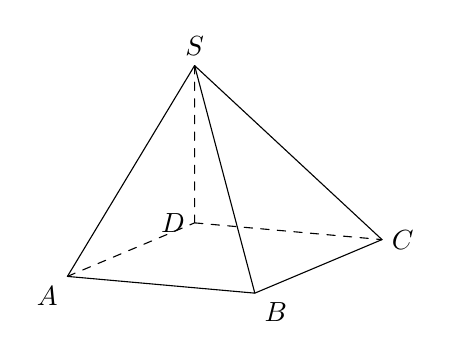
\begin{tikzpicture}[line cap=round,line join=round,scale=0.85]
  \coordinate (A) at (-2.4,0);
  \coordinate (B) at (0.4,-0.25);
  \coordinate (C) at (2.3,0.55);
  \coordinate (D) at (-0.5,0.8);
  \coordinate (S) at (-0.5,3.15);

  % Hidden back edges and the perpendicular altitude SD.
  \draw[dashed] (A)--(D) (D)--(C) (S)--(D);
  % Visible base edges and lateral edges.
  \draw (A)--(B)--(C);
  \draw (S)--(A) (S)--(B) (S)--(C);

  \node[below left] at (A) {$A$};
  \node[below right] at (B) {$B$};
  \node[right] at (C) {$C$};
  \node[left] at (D) {$D$};
  \node[above] at (S) {$S$};
\end{tikzpicture}
\end{center}
\nopagebreak[4]
\Needspace{4\baselineskip}
\textbf{解析}

\gksubpart{(1) 垂直关系}

取底面正方形顶点坐标 $D=(0,0,0)$、$C=(1,0,0)$、$B=(1,1,0)$、$A=(0,1,0)$。因 $SD\perp$ 底面，设 $S=(0,0,h)$。由 $SB^2=3$ 及 $DB^2=2$ 得 $h^2=1$，即 $h=1$。

此时 $\overrightarrow{BC}=(0,-1,0)$、$\overrightarrow{SC}=(1,0,-1)$，内积为 $0$，故 $BC\perp SC$。

\gksubpart{(2) 二面角}

\Needspace{5\baselineskip}
平面 $ASD$ 为 $x=0$，法向量可取 $\boldsymbol n_1=(1,0,0)$。平面 $BSC$ 的法向量可取 $\boldsymbol n_2=(1,0,1)$。两平面的锐二面角 $\theta$ 满足
\nopagebreak[4]
\[
\cos\theta=\frac{|\boldsymbol n_1\cdot\boldsymbol n_2|}{|\boldsymbol n_1||\boldsymbol n_2|}=\frac1{\sqrt2},
\]
故 $\theta=45^\circ$。

\gkanswer{答案（1）：$BC\perp SC$}

\gkanswer{答案（2）：$45^\circ$}

\end{answer}
\begin{answer}
\gksolhead{18}{}

\textbf{题目}：

$2003$ 年 $10$ 月 $15$ 日 $9$ 时，“神舟”五号载人飞船发射升空，于 $9$ 时 $9$ 分 $50$ 秒准确进入预定轨道，开始巡天飞行。该轨道是以地球的中心 $F_2$ 为一个焦点的椭圆。选取坐标系如图所示，椭圆中心在原点。近地点 $A$ 距地面 $200\,\text{km}$，远地点 $B$ 距地面 $350\,\text{km}$。已知地球半径 $R=6371\,\text{km}$。

(1) 求飞船飞行的椭圆轨道的方程；

(2) 飞船绕地球飞行了十四圈后，于 $16$ 日 $5$ 时 $59$ 分返回舱与推进舱分离，结束巡天飞行。飞船共巡天飞行了约 $6\times10^5\,\text{km}$，问飞船巡天飞行的平均速度是多少 $\text{km/s}$？（结果精确到 $1\,\text{km/s}$）
\nopagebreak[4]
\begin{center}% Qualitative schematic of the source diagram; geometry is not to scale.
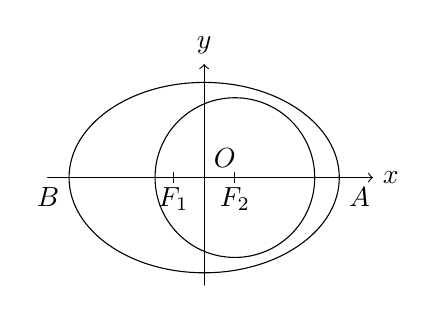
\begin{tikzpicture}[line cap=round,line join=round,scale=0.78]
  \coordinate (O) at (0,0);
  \coordinate (Fone) at (-0.5,0);
  \coordinate (Ftwo) at (0.5,0);
  \coordinate (A) at (2.2,0);
  \coordinate (B) at (-2.2,0);

  % Axes and the elliptical orbit.  No unprovided distances are asserted.
  \draw[->] (-2.55,0)--(2.75,0) node[right] {$x$};
  \draw[->] (0,-1.75)--(0,1.85) node[above] {$y$};
  \draw (O) ellipse (2.2 and 1.55);
  % The source depicts the Earth circle centered at F_2 and enclosing both O and F_1.
  \draw (Ftwo) circle[radius=1.3];

  % Foci are shown as short axis ticks, as in the source.
  \draw (-0.5,-0.08)--(-0.5,0.08);
  \draw (0.5,-0.08)--(0.5,0.08);
  \node[above right] at (O) {$O$};
  \node[below] at (Fone) {$F_1$};
  \node[below] at (Ftwo) {$F_2$};
  \node[below right] at (A) {$A$};
  \node[below left] at (B) {$B$};
\end{tikzpicture}
\end{center}
\nopagebreak[4]
\Needspace{4\baselineskip}
\textbf{解析}

\gksubpart{(1) 轨道方程}

\Needspace{5\baselineskip}
椭圆中心为原点，长轴在 $x$ 轴上，地心 $F_2$ 为右焦点。近地点距离给出 $a-c=6371+200=6571$；远地点距离给出 $a+c=6371+350=6721$。所以 $a=6646$、$c=75$，且
\nopagebreak[4]
\[
b^2=a^2-c^2=6646^2-75^2=44163691.
\]
轨道方程为 $\dfrac{x^2}{6646^2}+\dfrac{y^2}{44163691}=1$。

\gksubpart{(2) 平均速度}

\Needspace{5\baselineskip}
巡天飞行从 $15$ 日 $9$ 时 $9$ 分 $50$ 秒进入轨道开始，至 $16$ 日 $5$ 时 $59$ 分结束，历时 $20$ 小时 $49$ 分 $10$ 秒，即 $74950$ 秒。平均速度为
\nopagebreak[4]
\[
\frac{6\times10^5}{74950}\approx8.0053\,\text{km/s},
\]
精确到 $1\,\text{km/s}$ 为 $8\,\text{km/s}$。

若改从当日 $9$ 时发射时刻计时，历时为 $20$ 小时 $59$ 分，平均速度约为 $7.943\,\text{km/s}$；两种计时口径按题目要求精确到 $1\,\text{km/s}$ 均为 $8\,\text{km/s}$。此处按原文“进入预定轨道，开始巡天飞行”采用进入轨道时刻。

\gkanswer{答案（1）：$\dfrac{x^2}{6646^2}+\dfrac{y^2}{44163691}=1$}

\gkanswer{答案（2）：$8\,\text{km/s}$}

\end{answer}
\begin{answer}
\gksolhead{19}{}

\textbf{题目}：

某服装厂生产一种服装，每件服装的成本为 $40$ 元，出厂单价定为 $60$ 元。该厂为鼓励销售商订购，决定当一次订购量超过 $100$ 件时，每多订购一件，订购的全部服装的出厂单价就降低 $0.02$ 元。根据市场调查，经销商一次订购量不会超过 $500$ 件。

(1) 设一次订购量为 $x$ 件，服装的实际出厂单价为 $P$ 元，写出函数 $P=f(x)$ 的表达式；

(2) 当销售商一次订购 $400$ 件服装时，该服装厂获得的利润是多少元？（服装厂售出一件服装的利润 $=$ 实际出厂单价 $-$ 成本。）

\Needspace{4\baselineskip}
\textbf{解析}

\gksubpart{(1) 单价函数}

\Needspace{5\baselineskip}
订购量 $x$ 为正整数且不超过 $500$。不超过 $100$ 件时单价仍为 $60$ 元；超过 $100$ 件时，每增加一件使全部服装的单价减少 $0.02$ 元，因此
\nopagebreak[4]
\[
P=f(x)=\begin{cases}
60,&1\le x\le100,\\
60-0.02(x-100),&100<x\le500.
\end{cases}
\]
\gksubpart{(2) 订购400件时的利润}

当 $x=400$ 时，单价为 $60-0.02(400-100)=54$ 元，每件利润为 $54-40=14$ 元，总利润为 $400\times14=5600$ 元。

\gkanswer{答案（1）：$P=f(x)=\begin{cases}60,&1\le x\le100,\\60-0.02(x-100),&100<x\le500,\end{cases}\quad x\in\mathbb Z$}

\gkanswer{答案（2）：$5600$ 元}

\end{answer}
\begin{answer}
\gksolhead{20}{}

\textbf{题目}：

\Needspace{5\baselineskip}
下表给出一个“等差数阵”：

\nopagebreak[4]
\[
\begin{array}{|c|c|c|c|c|c|c|c|}
\hline
4 & 7 & (\quad) & (\quad) & (\quad) & \cdots & a_{1j} & \cdots \\ \hline
7 & 12 & (\quad) & (\quad) & (\quad) & \cdots & a_{2j} & \cdots \\ \hline
(\quad) & (\quad) & (\quad) & (\quad) & (\quad) & \cdots & a_{3j} & \cdots \\ \hline
(\quad) & (\quad) & (\quad) & (\quad) & (\quad) & \cdots & a_{4j} & \cdots \\ \hline
\cdots & \cdots & \cdots & \cdots & \cdots & \cdots & \cdots & \cdots \\ \hline
a_{i1} & a_{i2} & a_{i3} & a_{i4} & a_{i5} & \cdots & a_{ij} & \cdots \\ \hline
\cdots & \cdots & \cdots & \cdots & \cdots & \cdots & \cdots & \cdots \\ \hline
\end{array}
\]

其中每行、每列都是等差数列，$a_{ij}$ 表示位于第 $i$ 行第 $j$ 列的数。

(1) 写出 $a_{45}$ 的值；

(2) 写出 $a_{ij}$ 的计算公以及 $2008$ 这个数在等差数阵中所在的位置。

\begin{gktip}
原卷此处印作“计算公以及”，疑脱“式”字；本稿照录原文。
\end{gktip}

\Needspace{4\baselineskip}
\textbf{解析}

\gksubpart{(1) 计算 $a_{45}$}

\Needspace{5\baselineskip}
第一行公差为 $3$；第一列公差也为 $3$。第二行首项比第一行首项多 $3$，第二项比第一行第二项多 $5$，故每向右一列，行间公差增加 $2$。于是
\nopagebreak[4]
\[
a_{ij}=4+3(j-1)+(i-1)(2j+1)=2ij+i+j.
\]
所以 $a_{45}=2\cdot4\cdot5+4+5=49$。

\gksubpart{(2) 通项与数 $2008$ 的位置}

\Needspace{5\baselineskip}
要使 $a_{ij}=2008$，需
\nopagebreak[4]
\[
2ij+i+j=2008\iff(2i+1)(2j+1)=4017=3\cdot13\cdot103.
\]
\Needspace{5\baselineskip}
两个因数均为不小于 $3$ 的奇数。可取的有序因数对为 $(3,1339)$、$(13,309)$、$(39,103)$ 及其反序，因此
\nopagebreak[4]
\[
(i,j)\in\{(1,669),(6,154),(19,51),(51,19),(154,6),(669,1)\}.
\]

\gkanswer{答案（1）：$a_{45}=49$}

\gkanswer{答案（2）：$a_{ij}=2ij+i+j$；$2008$ 的位置 $(i,j)$ 为 $(1,669)$、$(6,154)$、$(19,51)$、$(51,19)$、$(154,6)$、$(669,1)$}

\end{answer}